% Six query paths into one contributed field, all of them stopping at the same
% crossing, and the one of the six the composer prints.
%
% Same idiom as figures/tikz/ch01-one-field.tex, which fixes it: 0.4pt strokes,
% the Straight Barb arrowhead, sans-serif scriptsize labels, square corners, no
% fills, black on white. The nearest relative is figures/tikz/ch07-the-walk.tex,
% which draws one of these six as a left-to-right walk and marks the step it
% cannot take with a cross; this figure keeps that cross and stacks six lanes
% against one shared crossing, because what chapter 15 adds to chapter 7 is not
% a new walk but the discovery that there were always several.
%
% Laid out as six lanes rather than six columns for the ordinary reason: the
% paths are of different lengths and read left to right, and six columns of a
% tree at this measure leaves no room for the labels. The seam is one vertical
% rule because here it genuinely is one crossing, which is the difference
% between this picture and the one at figures/tikz/ch14-the-climb-crosses.tex,
% whose comment block records why a single rule was wrong there.
%
% The field on the right is drawn solid and unreached. It exists, it is
% correctly declared, and nothing is wrong with it, which is the point of
% drawing it as an ordinary box rather than as a missing one.
%
% No quotation marks anywhere in this file, including this comment block. SPEC
% decision 30 puts the book in strict Ascii mode and the prose gate reads a
% literal quote character as a quotation mark on sight. Identifiers are bare.
%
% Bare tikzpicture (house style): the figure environment, caption and label
% live at the call site in the section file.
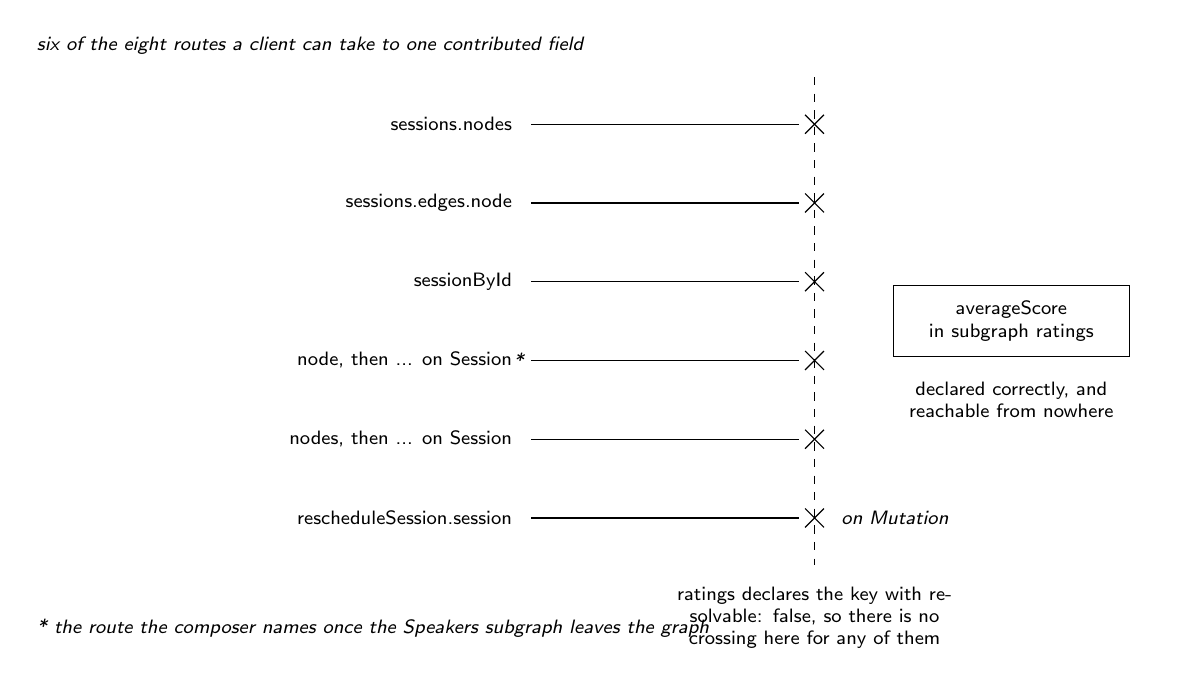
\begin{tikzpicture}[
  x=1mm, y=1mm,
  every node/.append style={font=\sffamily\scriptsize},
  route/.style={draw, line width=0.4pt},
  tick/.style={draw, line width=0.4pt},
  seam/.style={draw, line width=0.4pt, dashed},
  fieldbox/.style={draw, line width=0.4pt, minimum width=30mm,
    minimum height=9mm, align=center, inner sep=1pt},
  path/.style={anchor=east, align=right, inner sep=1pt},
  lane/.style={anchor=west, font=\sffamily\scriptsize\itshape},
  tag/.style={anchor=west, font=\sffamily\scriptsize\itshape, inner sep=1pt},
  spanlabel/.style={anchor=north, align=center, inner sep=2pt},
]

\node[lane] at (0,10)
  {six of the eight routes a client can take to one contributed field};

% ------------------------------------------------------ the six routes
% One lane each, path text on the left, a rule running right to the crossing.
% The cross at the end is chapter 7's buffer stop, and it is at the same x on
% every lane because it is the same crossing every time.
% Paths are written the way the composer writes them, dot-separated, rather
% than with a dash: a double hyphen in a TikZ node is text mode and LaTeX sets
% it as an en dash, which the book does not use anywhere.
\foreach \y/\p in {
    0/{sessions.nodes},
   -10/{sessions.edges.node},
   -20/{sessionById},
   -30/{node, then ... on Session},
   -40/{nodes, then ... on Session},
   -50/{rescheduleSession.session}}{
  \node[path] at (62,\y) {\p};
  \draw[route] (64,\y) -- (98,\y);
  \draw[tick] (98.8,\y-1.2) -- (101.2,\y+1.2);
  \draw[tick] (98.8,\y+1.2) -- (101.2,\y-1.2);
}

% Lane six is on the mutation root rather than on the query root.
\node[tag] at (103,-50) {on Mutation};

% --------------------------------------------------------- the crossing
\draw[seam] (100,6) -- (100,-56);
\node[spanlabel, text width=46mm] at (100,-58)
  {ratings declares the key with resolvable: false, so there is no crossing
   here for any of them};

% ------------------------------------------------------------ the field
\node[fieldbox] (field) at (125,-25) {averageScore\\in subgraph ratings};
\node[spanlabel, text width=34mm] at (125,-32)
  {declared correctly, and reachable from nowhere};

% ------------------------------------------- which one gets reported
% A mark and a legend rather than a change of line style. All six lanes are the
% same walk failing the same way, so nothing about the route itself may be
% drawn differently; what is different is only that this one reached the
% report. Solid against dashed already carries the crossing in this figure and
% the arrowhead already carries a blocked step in ch07-the-walk.tex, so neither
% is available here.
\node[tag, anchor=east] at (63.5,-30) {*};
\node[lane] at (0,-64)
  {* the route the composer names once the Speakers subgraph leaves the graph};

\end{tikzpicture}
